%----------------------------------------------
\section{Introduction} \label{sec:intro}
%----------------------------------------------

As alluded to earlier in chap.~\ref{c:intro}, flares manifest differently across various wavelengths. It is known that the foot-points of the post-flare loops are observed in hard X-rays (due to electrons) and $\gamma$~rays (due to ions). However, the post-flare loops themselves are observed in soft X-ray and Extreme Ultraviolet (EUV) \citep{fletcher11,TriBC_2004,tripathi06}. The corresponding white light and Near Ultraviolet (NUV) counterparts are believed to arise due to changes in ionization and local opacity in the photospheric and chromospheric heights. %These are usually \textbf{detected?} in some of the most impulsive signatures of flares \citep{watanabe17,hudson06}. 
The NUV and white light emission have also been demonstrated to be co-spatial and co-temporal with hard X-ray \citep{hudson92, oliverso12}. 

One of the major puzzling aspects regarding the origin and energetics of solar flares is the origin of the white light (WL) continuum. According to the standard model of flares, the energetic electrons are accelerated along the loops and are stopped via numerous collisions and thermalization when the ambient medium has enough density, usually known as the `thick target' model \citep[see][for further details]{brown73,benz17,fletcher11}. It is believed that such densities are already present within the chromosphere, explaining the co-spatiotemporal nature of WL and Hard X-ray emission. The theoretical estimations, on the other hand, predict that parts of the WL emission may originate in the upper photosphere, i.e., depths which are inaccessible to electrons in the standard `thick-target' model. 

There have been various attempts to modify the thick target model to account for various observations from solar flares, e.g., a warm target model \citep{kontar15,kontar19}, local re-acceleration of electrons \citep{brown73}, acceleration of protons along with electrons which are expected to penetrate deeper. There were also attempts to explain the source of WL with photospheric `back-warming' \citep{metclaff90}, where the upper photosphere is ionized via energy transported radiatively from the chromosphere. There have been several observations where the WL emission has been associated with enhancement observed in the 2832~{\AA} continuum of IRIS SJI \citep{heinzel14,kleint16,kleint17,kowalski17,kowalski19}. 

In this chapter, we discuss the X-class flare recorded by the Solar Ultraviolet Imaging Telescope \citep[SUIT;][]{suit,suit_main} on board Aditya-L1 \citep{adityal1} on February 22, 2024. This is the first flare that was localized and observed with the onboard flare detection module. %Continuum bright kernels were observed in the red wing (283~nm) and blue wing (276~nm) of the Mg window. To the best of our knowledge, this is the first observation of continuum enhancement of the blue wing of Mg window. 
The rest of the {\bf chapter} is structured as follows: in \S\ref{obs}, we discuss the observations of the flare and the dataset used for its study. \S\ref{res} we discuss the data analysis and results. Finally, in \S\ref{sec:disc}, we summarize, conclude and discuss the importance of these observations in flare studies. 
%In \S\ref{sec:bright_ker}, we discuss the observations specifically related to the penumbral bright kernels and how they compare across various wavelengths. In \S3, We summarize our findings and discuss the implications it can have regarding our understanding of the origin of WL emission is solar flares.
%-----------------------------------------------
\section{Observations and Data}\label{obs} 
%-----------------------------------------------
Active Region NOAA 13590 appeared on Feb. 18, 2024, at the northeast limb of the solar disk. On Feb. 22, 2024, it was located at N17E26 with $\beta\gamma\delta$ configuration and produced multiple flares, including the M4.8, X~1.7 and X6.3.% , an M4.8 aflare peaking around $\sim$ 06:32 UT, 20:46 UT and an X6.3 flare that peaked $\sim$ 22:34 UT . 

Using the onboard flare detection algorithm based on intensity thresholding \citep{flare_det}, SUIT detected, localized and observed the X6.3 flare in flare mode. SUIT instrument carries 11 filters (8 narrow bands and 3 broad bands) tuned to observe the solar photosphere and chromosphere at various wavelengths in 200-400~{nm} wavelength range (see Table~\ref{tab:science_filters}). SUIT provides images at a pixel size of 0.7{\arcsec}. The four out of eight narrow band filters are tuned to observe the \ion{Mg}{2} blue wing continuum (NB2), \ion{Mg}{2}~k (NB3), \ion{Mg}{2}~h (NB5) and \ion{Mg}{2} red wing continuum (NB5). The NB6 and NB7 continuum filters are towards the blue and red sides of the Balmer jump (364.5~nm), respectively. 

It provides both full disk and region of interest (ROI) observations as per the observational sequence being used. While in regular observations, the RoI is defined using ground commands, flare mode automatically defines the RoI based on the detected location and observes in the eight narrowband filters. Under this observation mode, the temporal cadence is $\approx$1~min. SUIT did not detect the X1.7 as the spacecraft was off-pointed for the stellar calibration sequence. The X6.3 flare that SUIT detected started at 22:08~UT and peaked at 22:34~UT. In the flare mode, it was observed in all eight narrowband filers. The flares were also observed by GOES, {\it SDO}/AIA, {\it SO}/STIX, GONG H$\alpha$. In this study, we have used AIA~1600 \& 1700~{\AA}, GONG~H$\alpha$ images and full disk integrated GOES soft-ray (1{--}8~{\AA}) and STIX Hard X-ray (25{--}50~keV) along with SUIT observations.

%-----------------------------------------------
\begin{figure*}[!h]
    \centering
    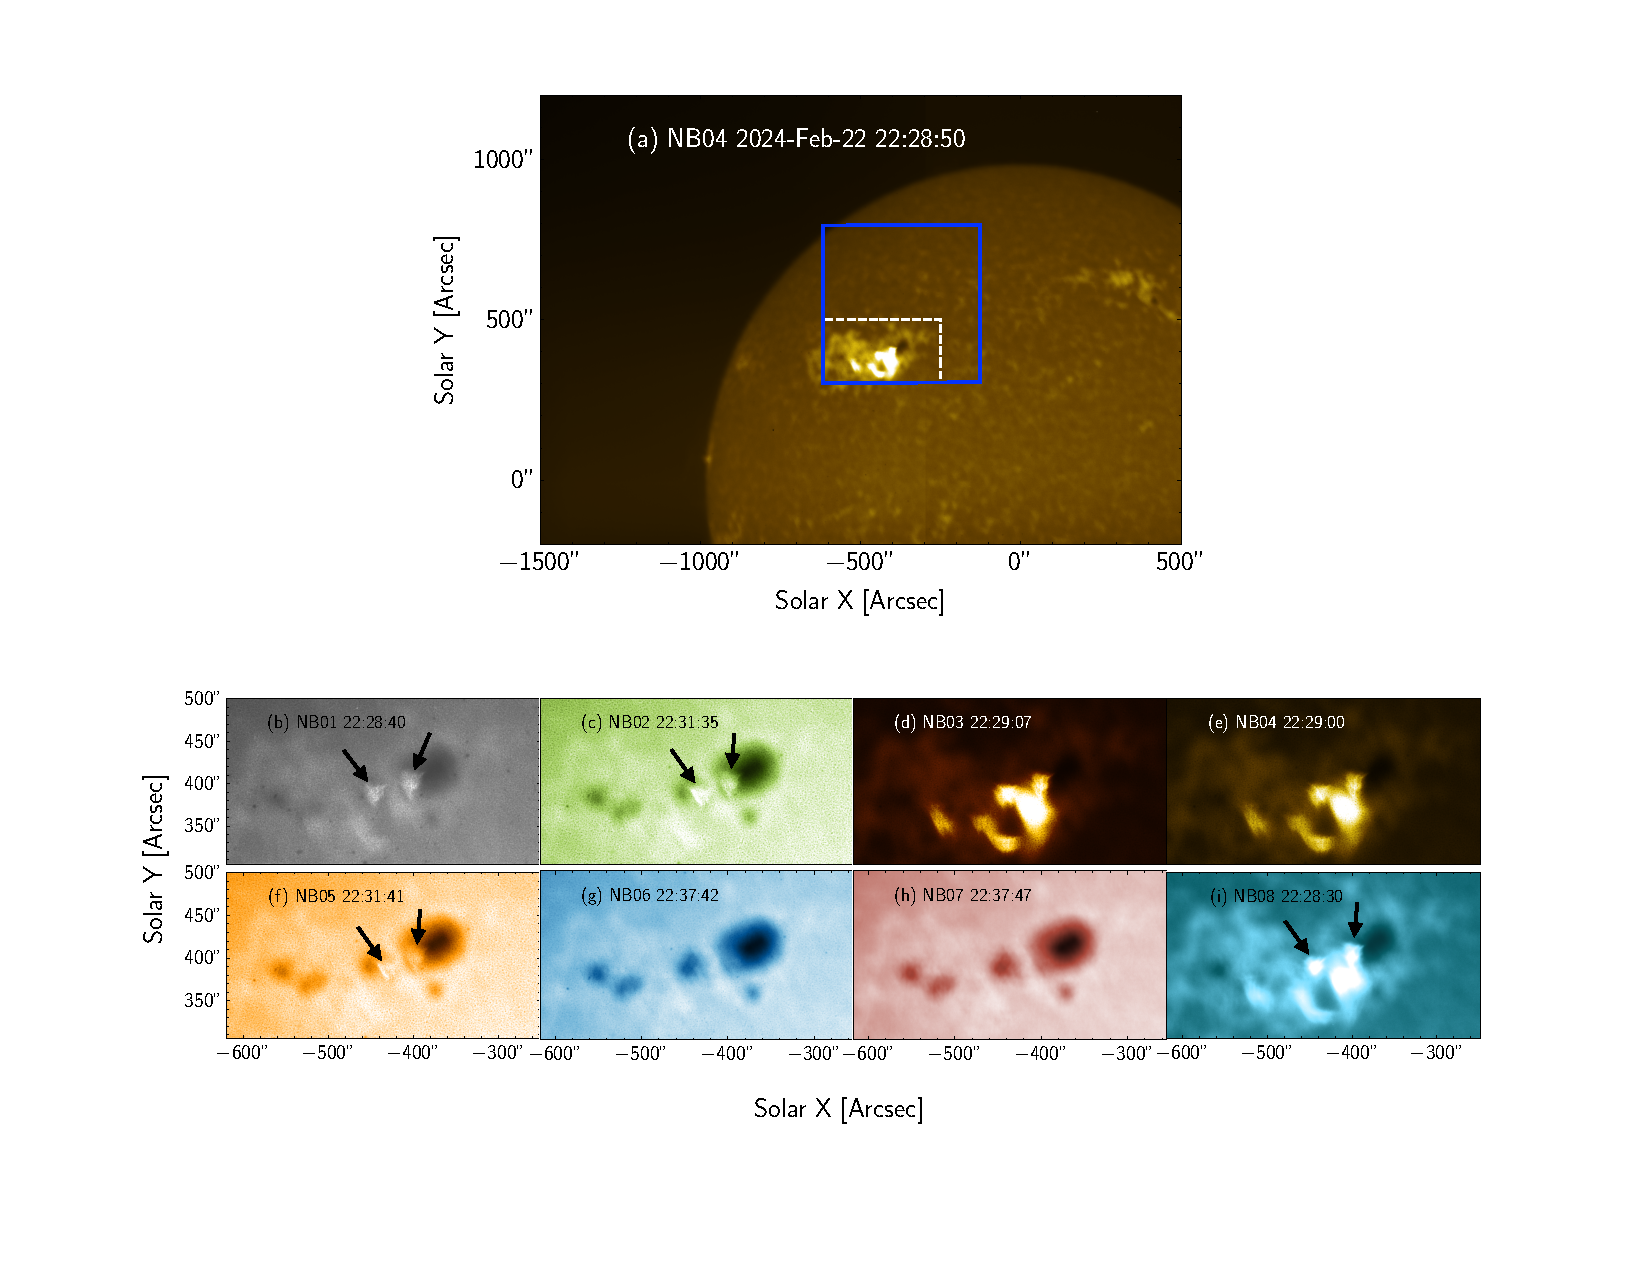
\includegraphics[trim = {2cm 2.5cm 2cm 1.8cm}, clip, width=0.9\textwidth]{Figures/feb_22nd/suit_roi_all_peak.pdf} 
    \caption[SUIT observation of the flare in all NB filters at their respective peaks]{(a) Parts of the full-disk (2k$\times$2k) observation in NB4 (\ion{Mg}{2}~h) showing the flaring region and sunspot. The over-plotted blue box shows the RoI localized by the onboard flare detection algorithm, and the white dashed box locates the region used for the subsequent analysis. (b) SUIT Narrowband images recorded at the peak of flares in the respective filters. The size of the images corresponds to the white-boxed region shown in panel a. The arrows mark the two bright umbral kernels.}
    \label{fig:flare_obs}
\end{figure*}
%-----------------------------------------------

\newpage

%-----------------------------------------------
\section{Data Analysis and results}\label{res}
%-----------------------------------------------

%-----------------------------------------------
%\begin{figure}
\begin{wrapfigure}{l}{0.5\textwidth}
    \centering
    \hspace{-1cm}
   \includegraphics[trim={1.5cm 2.5cm 1.5cm 1cm},clip,width=\linewidth]{Figures/feb_22nd/suit_roi_aia_peak.pdf}
    \caption[AIA and GONG observations of the flare]{Co-aligned and co-registered AIA 1600, 1700~{\AA} and GONG H{$\alpha$} observation near the NB3 peak in a, b and c, respectively. The over-plotted contours show 60\% of the peak intensity observed in NB3.}\label{aia}
\end{wrapfigure}
%\end{figure}
%-----------------------------------------------

Figure~\ref{fig:flare_obs}.a displays shows a cutout of the full-disk (2k$\times$2k) image taken in NB4 (\ion{Mg}{2}~h) filter. The over-plotted blue box shows the region of interest automatically defined by the onboard flare detection algorithm. As we can see, the auto-defined RoI fully covers the flare. The flare detection algorithm is designed to define the RoI, which is centred on the flaring region. In the current observation, we can see that the RoI is not properly centred at the flare. However, since then, various parameters of the flare detection and localization algorithm have been tweaked to achieve better detection and localization. The white dashed box locates the region we have considered for further study in this {\bf chapter}. Fig.~\ref{fig:flare_obs}.{b-i} displays the flares in each narrow band filter at their respective peak. The field of view (FOV) corresponds to the dashed white box in panel a. As can be seen, the flare is observed in all the narrow band filters of SUIT, including the two flare kernels observed as penumbral brightening, which are located by black arrows. % in d during the respective peaks of NB2 and NB5 (marked by black arrows in Fig.~\ref{fig:flare_obs}c and f respectively).
%-----------------------------------------------
\begin{figure*}
    \centering
    \includegraphics[trim={0.2cm 2.5cm 1cm 3.5cm},clip,width=\linewidth]{Figures/feb_22nd/suit_roi_nb3_peak.pdf}
    \caption[SUIT observation of the flare in all NB filters at NB3 peak]{Flare as observed in all narrow band filters at the time of peak intensity in NB3. The over-plotted black contours show 60\% of the peak intensity observed in NB3.}
    \label{fig:flare_nb3_peak}
\end{figure*}
%-----------------------------------------------

In Fig.~\ref{fig:flare_nb3_peak}, we plot the flare as observed in each narrow band filter at the peak intensity in NB3(\ion{Mg}{2}~k).%channel at around $\sim$ 22:28-22:29 UT. 
The over-plotted black contours represent 60\% of the peak intensity observed in NB3. The features observed in NB8 (\ion{Ca}{2}~h) are very similar in morphology to those in NB3 and NB4. While there appears to be a hint of such features in other continuum channels, it is not clearly discernible. 

%-----------------------------------------------
\begin{figure*}
    \centering
    \includegraphics[width=0.9\textwidth,trim={1cm 2cm 1cm 4.2cm},clip]{Figures/feb_22nd/lc_4.pdf}
    \caption[Comparison of SUIT NB lightcurve with other observatories]{Light curves obtained over the contoured region from AIA 1600 (blue dashed), AIA 1700~{\AA} (black do-dashed), NB3 (black dotted), NB4 (green dot-dashed), NB8 (magenta dashed), NB2 (blue dotted), NB5 (green dashed), NB1 (green triangles), NB6 (magenta squares) and NB7 (blue dotted) as labelled. For comparison, we have also over-plotted the light curves obtained from coaligned GONG H-alpha observations (blue squares) in panel (a), full-sun integrated GOES/SXR in 1{--}8~{\AA} (red solid) and STIX/HRX (black dashed) in panel (c).}
    \label{fig:flare_lc_suit}
\end{figure*}
%----------------------------------------------- 

To compare the SUIT observations with those from AIA and H$\alpha$, in Fig.~\ref{aia}, we plot display AIA~1600 (panel a), AIA~1700 (panel b) and GONG-H$\alpha$ recorded at near simultaneous time to the peak of NB3 observations. The over-plotted contours are the same as those in Fig~\ref{fig:flare_nb3_peak}. These images clearly reveal the presence of clear signatures of the flare kernels in AIA UV and H$\alpha$ observations, co-spatial to the NB3 (\ion{Mg}{2}~k) observations.

In order to understand the temporal evolution of the flare, we plot the lightcurves in Fig.~\ref{fig:flare_lc_suit} obtained from various filters of SUIT, GOES, STIX, AIA 1600 \& 1700, and GONG H$\alpha$, as labelled. Note that the GOES and STIX lightcurves are full Sun integrated, whereas those for other observations are obtained over the contoured region Figs.~\ref{fig:flare_nb3_peak}~\&~\ref{aia}, and normalized to their respective max intensities. The vertical dotted black line across all the panels locates the peak intensity in NB3. 

The lightcurves reveal that the flare peaks in all the SUIT channels (except NB6 and NB7), AIA 1600 \& 1700, H$\alpha$ and STIX before it achieves its maximum intensity in GOES. The STIX peak coincides with that in SUIT NB1, NB3, NB4, NB8 as well as AIA and H$\alpha$. Note that SUIT NB3, NB4 and NB8 primarily observe the chromospheric signatures, similar to GONG H$\alpha$. Fig.~\ref{fig:flare_lc_suit}.b, shows that the lightcurves of NB3, NB4, and NB8 peak at the same time around $\sim$ 22:29~UT, which is similar to that H$\alpha$. However, NB8 and {\it GONG}-H$\alpha$ show less contrast variation ($\sim$ 40\% change for NB8 (\ion{Ca}{2} h) and GONG H$\alpha$, compared to the $\sim$ 80\% change for NB3 (\ion{Mg}{2} k) and NB4 (\ion{Mg}{2} h)) than that shown by NB3 and NB4. This may be attributed to the larger enhancement in the continuum in NB8 (\ion{Ca}{2}) and H$\alpha$ than that in \ion{Mg}{2}.

Figure~\ref{fig:flare_lc_suit}.c shows that the lightcurves of SUIT NB2 and NB5 (blue and red wing of \ion{Mg}{2}) peak about 3 minutes after the NB3 peak (also STIX hard X-ray peak). This is also apparent in the images shown in Fig~\ref{fig:flare_obs}. Moreover, unlike other lightcurves, NB6 and NB7 lightcurves do not show a gradual increase and decrease. Instead, they exhibit a rather sharp rise, albeit very small ($\sim$ 0.03\%), in intensity during the impulsive phase of the flare.

%%--------------------------------------------
\section{Summary and Discussion}\label{sec:disc}
%%--------------------------------------------

In this {\bf chapter}, we have performed a multi-wavelength study of the X-6.3 flare observed on Feb 22, 2024, using the observations recorded by SUIT, AIA, STIX and GONG. Moreover, this is the first flare detected and localized by the onboard algorithm for flare identification on SUIT and observed in flare mode. Below we summarize the obtained results.
\begin{itemize}
    \item The flare is observed in all narrow band filters of SUIT. The flare was also observed in AIA 1700 and 1600, GONG~H$\alpha$, GOES soft X-rays (SXR) and STIX hard X-rays (HXR).
    \item The flare peak in all SUIT channels (except NB6 and NB7) and those in AIA 1600 \& 1700~{\AA}, GONG~H$\alpha$ and STIX HXR observations and is $\sim$ 5 minutes prior to the GOES SXR peak. The flare peaks are observed in NB6 and NB7 after $\sim$ 3 minutes after the GOES SXR peak.
    \item The flare peak in NB3 and NB4 coincides with that in AIA 1600 \& 1700~{\AA} and STIX 25{--}50~keV observations.
    \item The flare attains its peak in NB2 and NB5, blue and red wing of \ion{Mg}{2} lines, after about 3 minutes it does in NB3.    
\end{itemize}

The results demonstrate that the flare signatures detected by SUIT in all its narrow band channels are very tightly related to HXR observations recorded by STIX. These results highlight the first {\suit} observations of an X-class flare. The observations of flare kernels and enhancement in the intensity in the red wing of the \ion{Mg}{2} window, i.e., NB5 is similar to those observed by \cite{kowalski19,kowalski17,kleint17} using the observations recorded by the Interface Region Imaging Spectrometer \citep[IRIS,][]{iris}. For the flare studied here, we also detect the bright kernels and intensity enhancements in the blue wing of the Mg window, i.e., in NB2 filter. To the best of our knowledge, this is the first such observation in the blue wing of \ion{Mg}{2}. Unfortunately, we can not comment on the spectral nature of the bright kernels as SUIT is only an imager. Further exploration is necessary to comment on the spectral nature of the bright kernels and their possible origin. It is important to highlight that in the observation reported by \cite{kowalski19}, the appearance of flare kernel and intensity enhancement in SJI recorded at 2832~{\AA} (similar to SUIT NB5 filter) corresponded with a plethora of photospheric absorption lines, mostly \ion{Fe}{2}, turning into emission, which was attributed to photospheric heating.  would  Therefore, no such analysis was possible. 